\documentclass{article}

\usepackage{a4wide}
\usepackage[utf8]{inputenc}
\usepackage[T1]{fontenc}
\usepackage[french]{babel}
\usepackage[babel=true]{csquotes} % guillemets français
\usepackage{graphicx}
\graphicspath{{Images/}}
\usepackage{color}
\usepackage{hyperref}
\hypersetup{colorlinks,linkcolor=,urlcolor=blue}

\usepackage{amsmath}
\usepackage{amssymb}


\title{UnivMap}
\author{Damien LAOUSSING, Dylan CHERRIER, L3 informatique}
\date{\today}

\begin{document}

\maketitle %% pour écrire le titre


%% Le résumé:
\begin{abstract}
  UnivMap est une application mobile iOS et Android destinée au nouveau
  étudiant afin de les aider à se repérer au sein de l'Université de la Réunion.
\end{abstract}


\section{Introduction}
\label{section:intro} % pour faire référence à la section ailleurs (\ref{...} voir plus bas)

Dans le cadre du projet de l'unité d'enseignement "Développement pour Mobiles", nous avons décidé de développer
une application iOS et Android, visant les nouveaux étudiants de l'Université de la Réunion.

Beaucoup d'étudiants découvrant leurs nouveau campus, sont souvent perdu pour retrouver leurs chemin. Par conséquent,
ils arrivent souvent en retard dans leur cours et perdent ainsi leur qualité d'apprentissage.
Aujourd'hui, afin de répondre aux besoin de ces nouveaux étudiants, nous allons vous présenter l'application UnivMap.

Dans un premier temps, nous allons voir une description générale de l'application, puis nous verrons
l'architecture du code. Ensuite, nous aborderons les difficultés rencontrés durant le développement
du projet pour enfin terminer par une conclusion.

\section{Description générale de l'application}


L'application possèdes trois onglets : la carte de l'Université, le calendrier des cours ainsi que des options.
La carte intègres des fonctionnalités permettant l'affichage des enseignements sous formes de cercle coloré, De plus,
des boutons sont à la disposition de l'utilisateur afin de parcourir automatiquement ces cercles.
Le calendrier permet d'afficher sous d'une liste le planning.
Les options inclus la possibilité de changer la couleur du fond de l'application et de changer la langues.

L'application utilise principalement la carte de l'API \textit{Mapbox}~\cite{mapboxDoc} développé par l'entreprise
du même nom sur les bases du logiciel libre et sur les données d'\textit{OpenStreetMap}~\cite{openstreetmapDoc}.
La persistance de donné de notre application est gérer par le système interne mais aussi par la plateforme
de Google, \textit{Firebase}~\cite{firebaseDoc}.



\newpage %% Passer a une autre page



\subsection{Présentation de la carte et annoations des points}

Tout d'abord, UnivMap requiert une connexion internet afin de géolocaliser son utilisateur mais aussi
pour récupérer des données indispensables à son fonctionnement (map, liste des cours, ect...). Au lancement,
l'utilisateur se retrouve sur l'onglet de la carte et voit tous les positions des cours. En cliquant sur l'un d'eux,
un pop-up apparait affichant les informations essentielles du cours (nom du cours, nom de l'enseignant, salle et horaire).

\begin{itemize}
    \item Point bleu : les marqueurs de couleur bleu représente la position des cours qui n'ont pas encore commencer.

    \item Point orange : le marqueur de couleur orange représente la position du cours qui commençera dans
    moins de deux heures.

    \item Point rouge : le marqueur de couleur rouge représente la position du cours qui a déjà débuté.

    \item Point gris : le marqueur de couleur gris représente la position du cours terminé
\end{itemize}

\vspace{10pt}   %espace

\begin{center}
    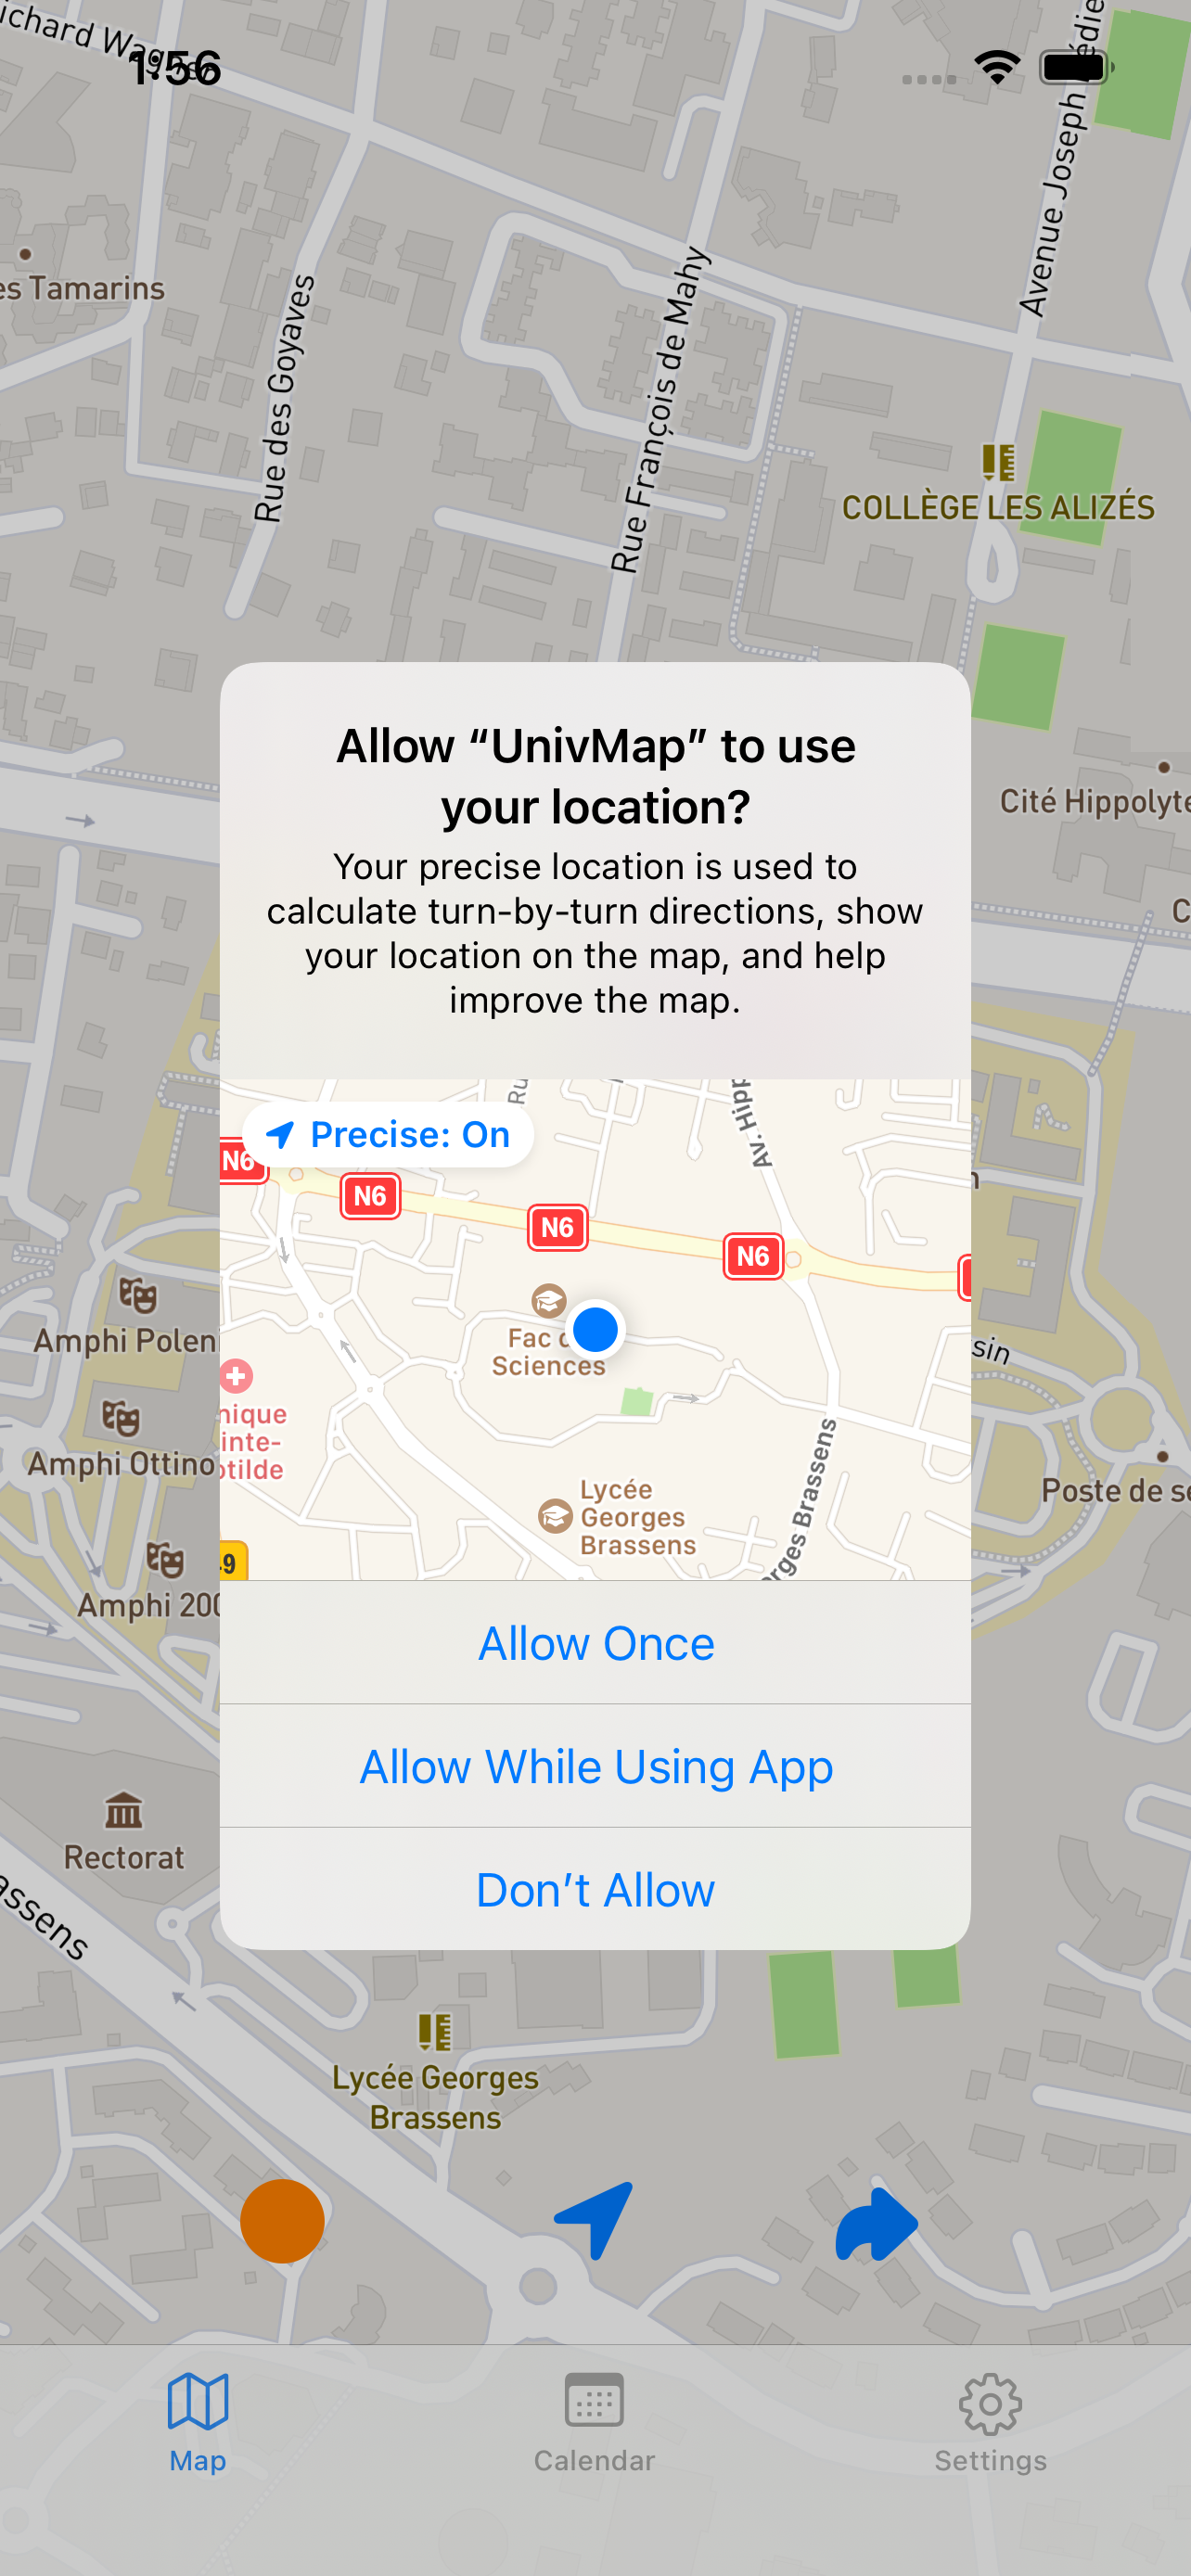
\includegraphics[width=45mm, scale=0.5]{allowUserLocation.png}
    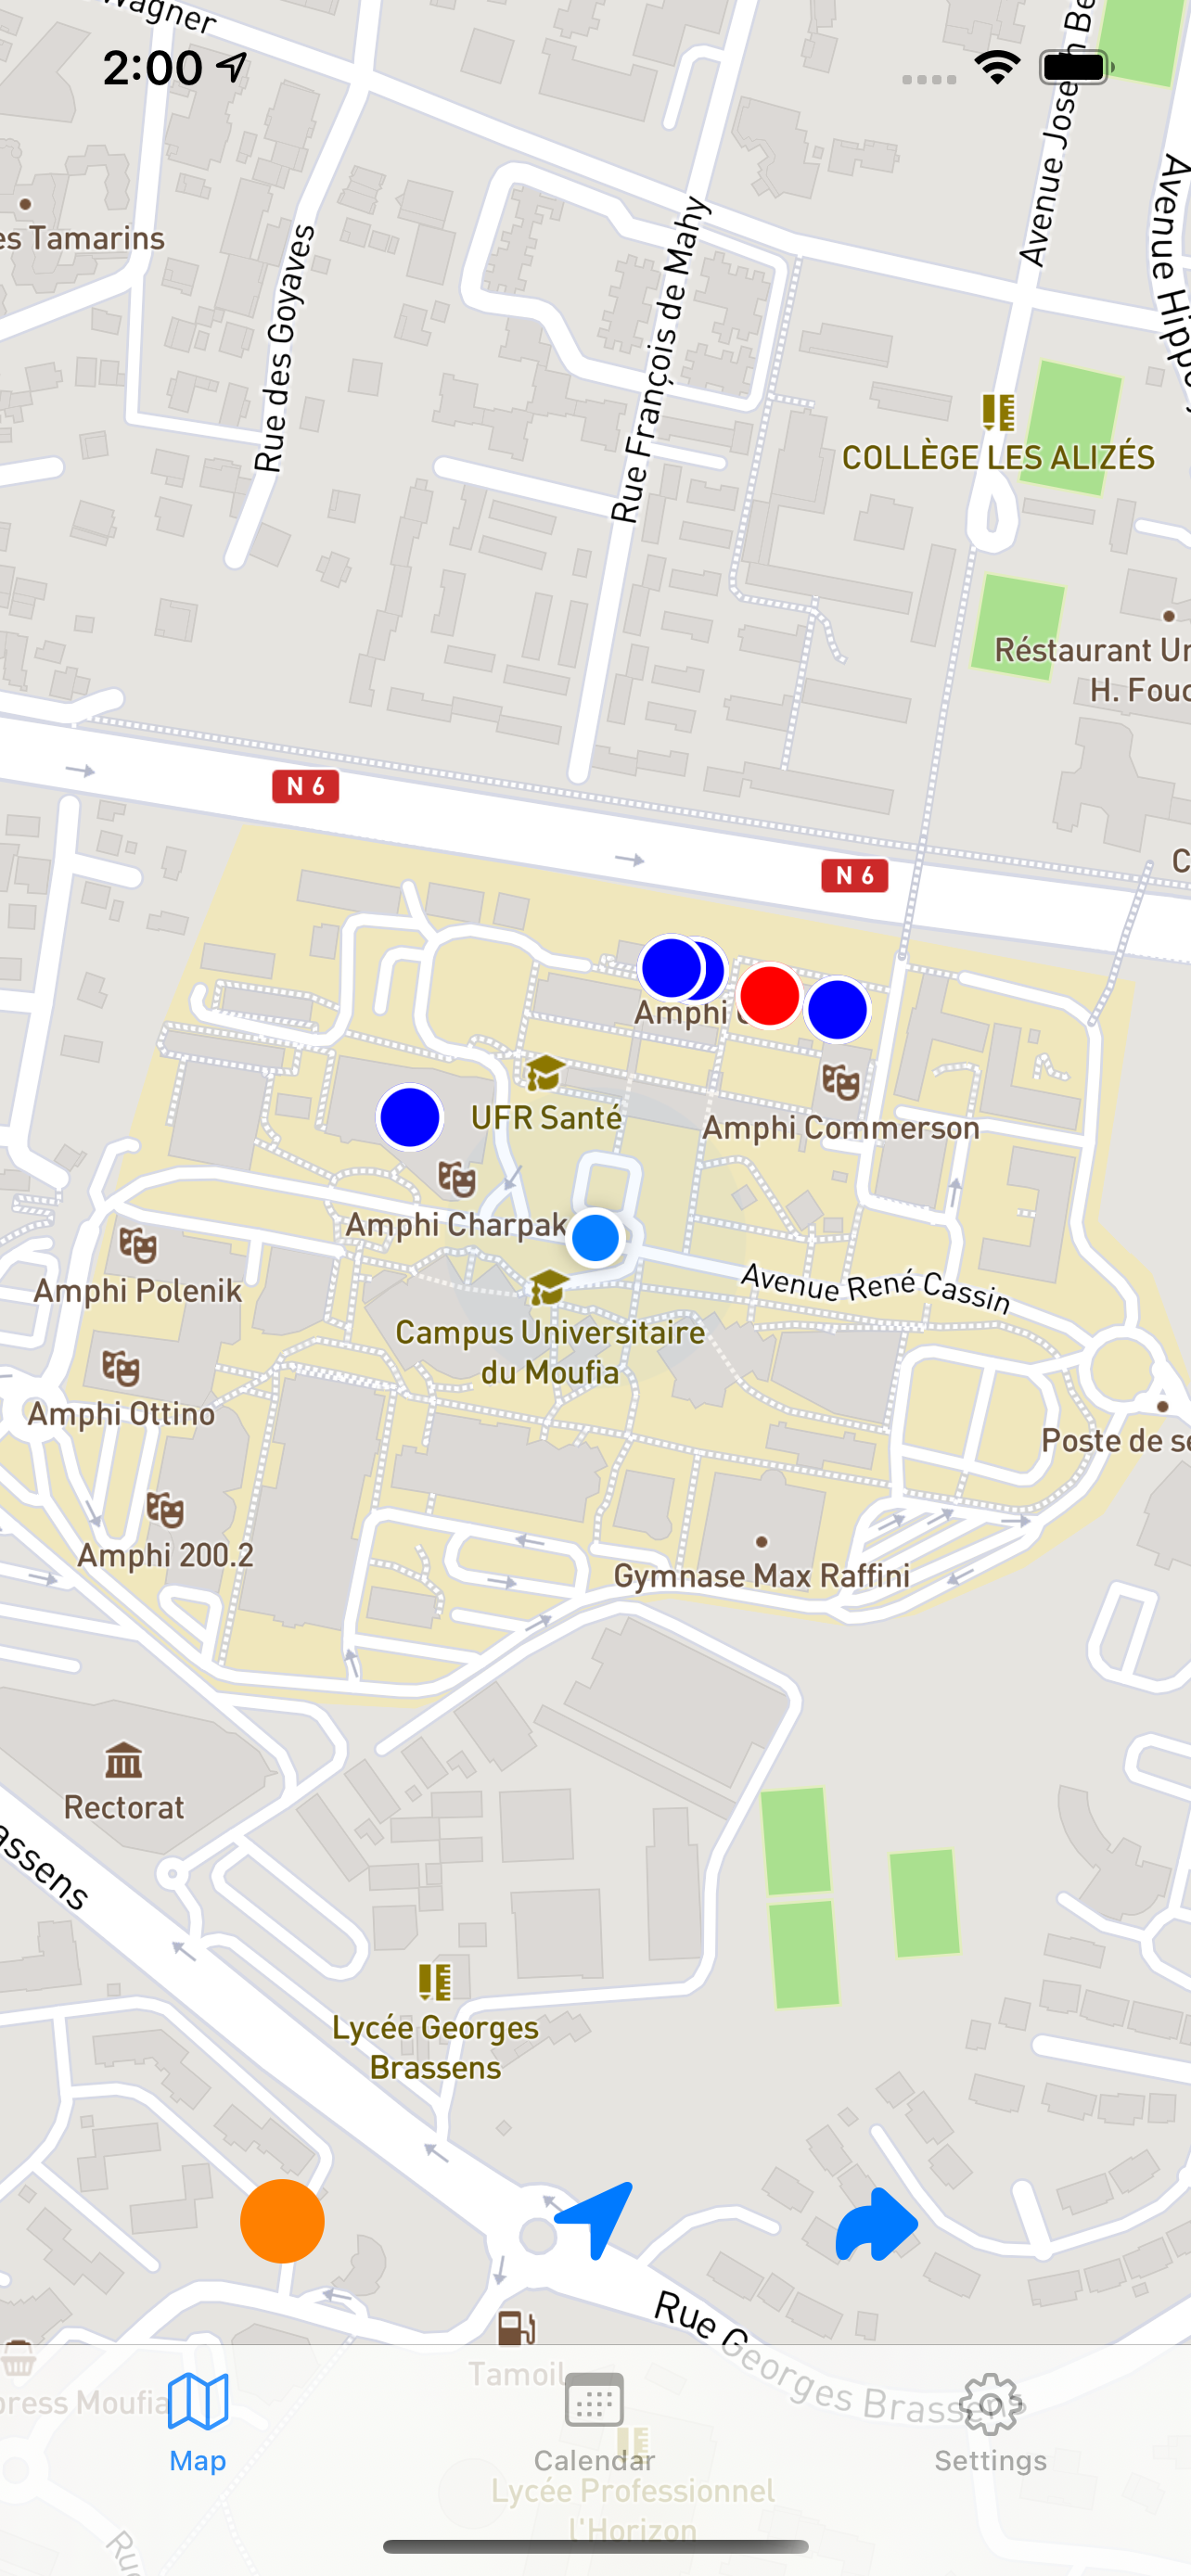
\includegraphics[width=45mm, scale=0.5]{map.png}
    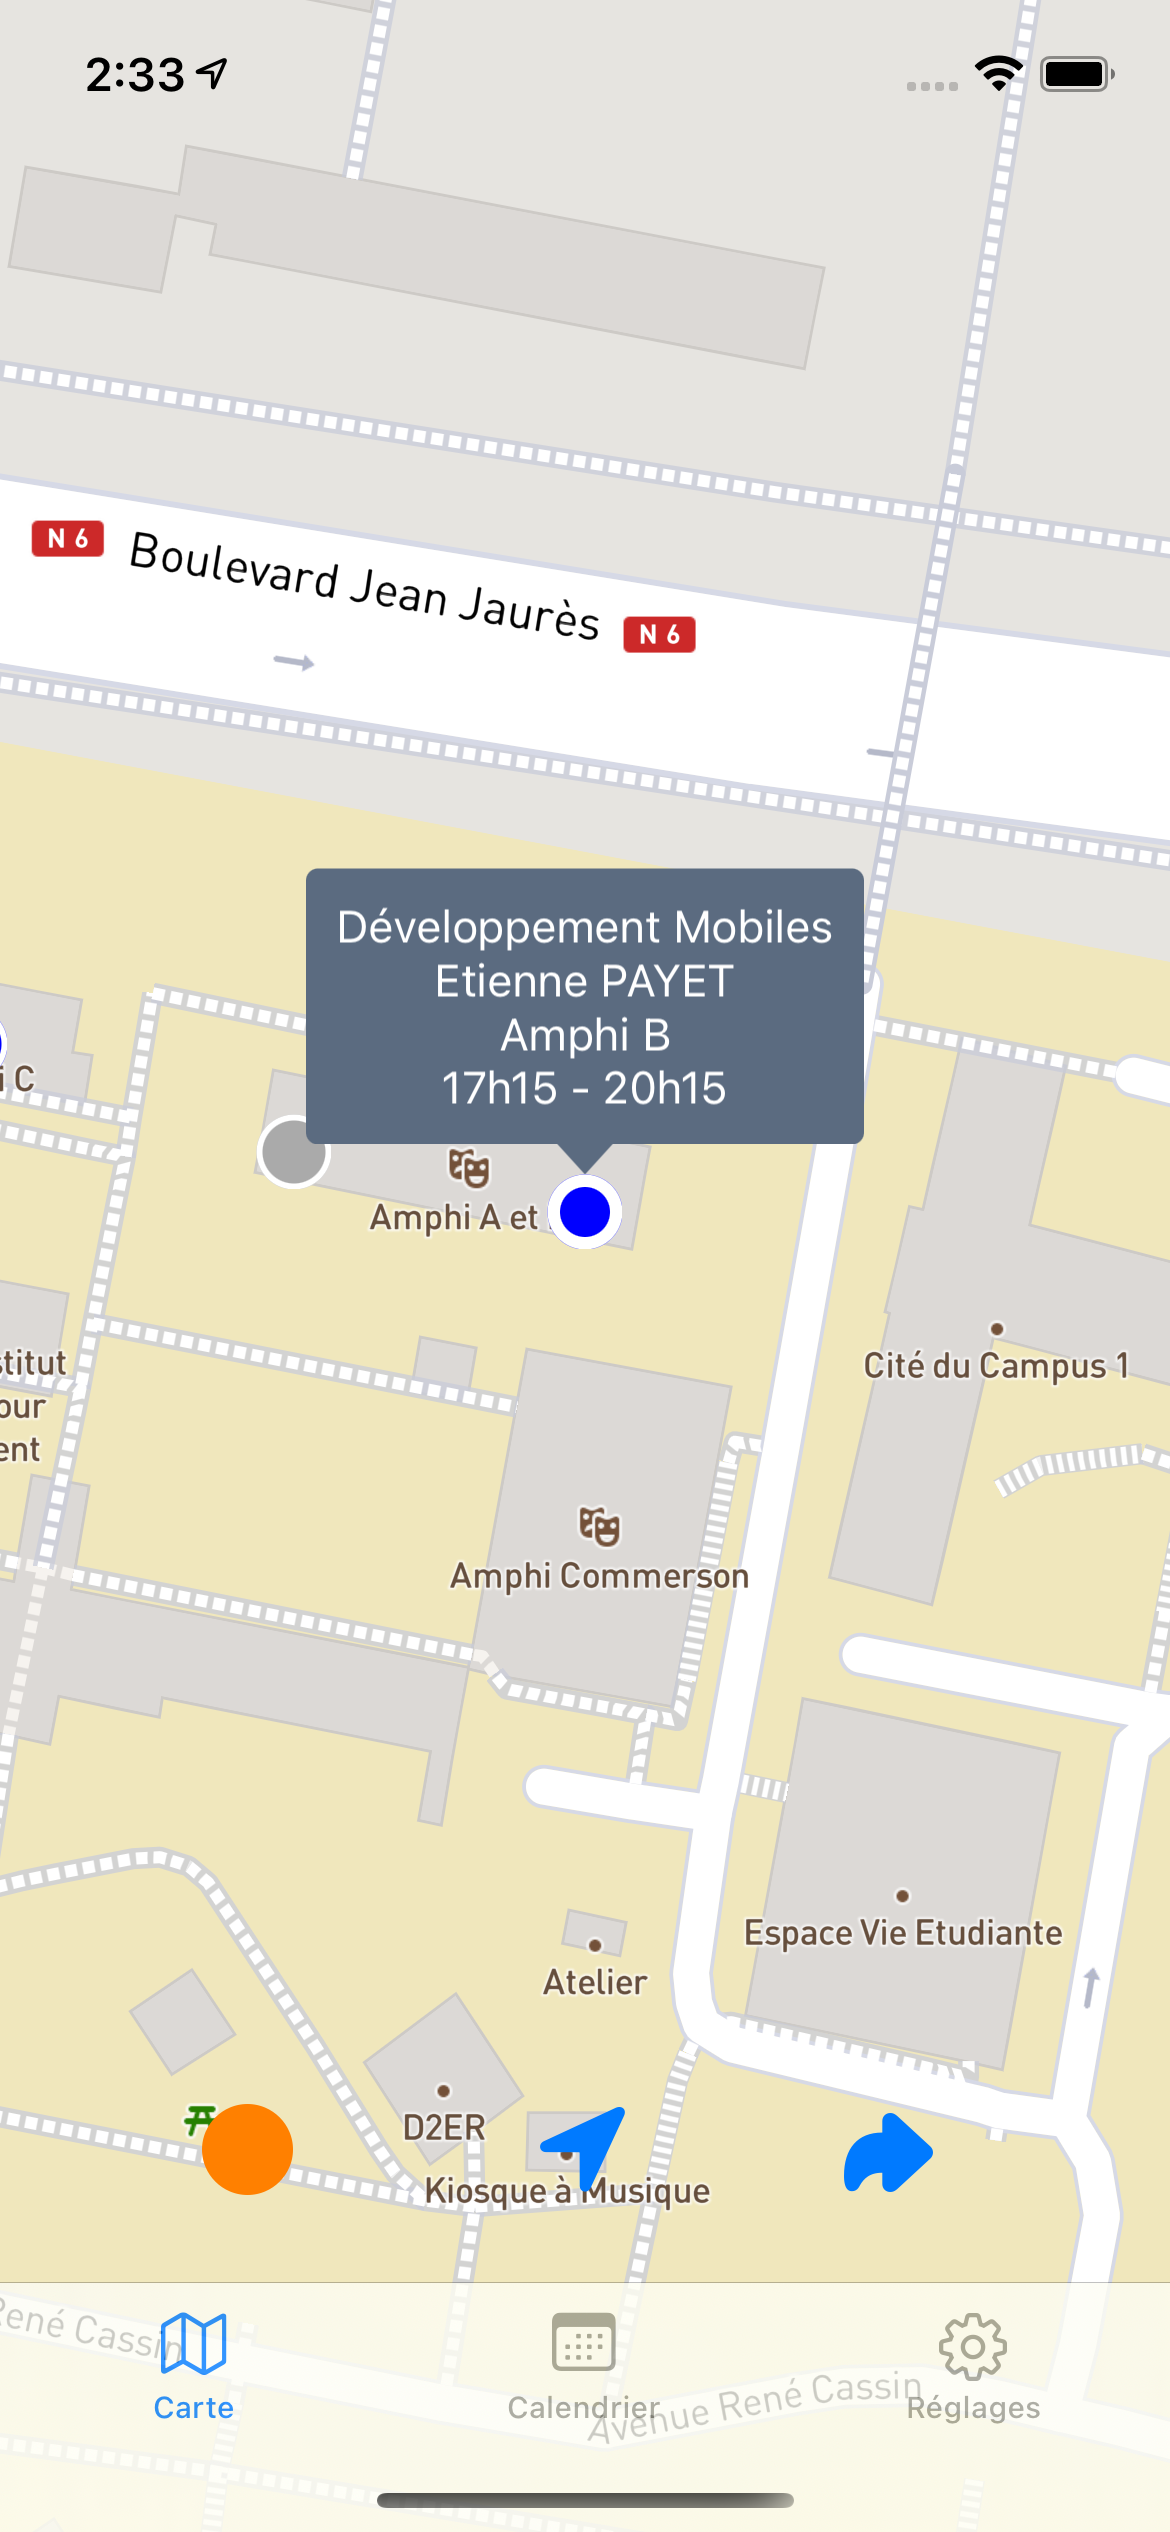
\includegraphics[width=45mm, scale=0.5]{point_bleu.png}
\end{center}

Les trois boutons du bas permet de changer la vue de la caméra.

\begin{itemize}
    \item Bouton de gauche : parcours les cours qui débuterons prochainement

    \item Bouton du milieu : centre sur la position de l'utilisateur.

    \item Bouton de droite : permet de parcourir parmis tous les cours sur la map.
\end{itemize}



\newpage %% Passer a une autre page



\subsection{Calendrier : la liste des cours}

L'onglet calendrier permet l'affichage de tous les cours trier par ordre croissant selon l'heure. Pour récupérer ces
données, l'application utilise \textit{Firebase}~\cite{firebaseDoc}, un service d'hébergement en NoSQL
développer par Google. En selectionnant le cours, l'application nous redirige vers une nouvelle vue,
affichant la position exacte de celui-ci.

\vspace{10pt}   %espace

\begin{center}
    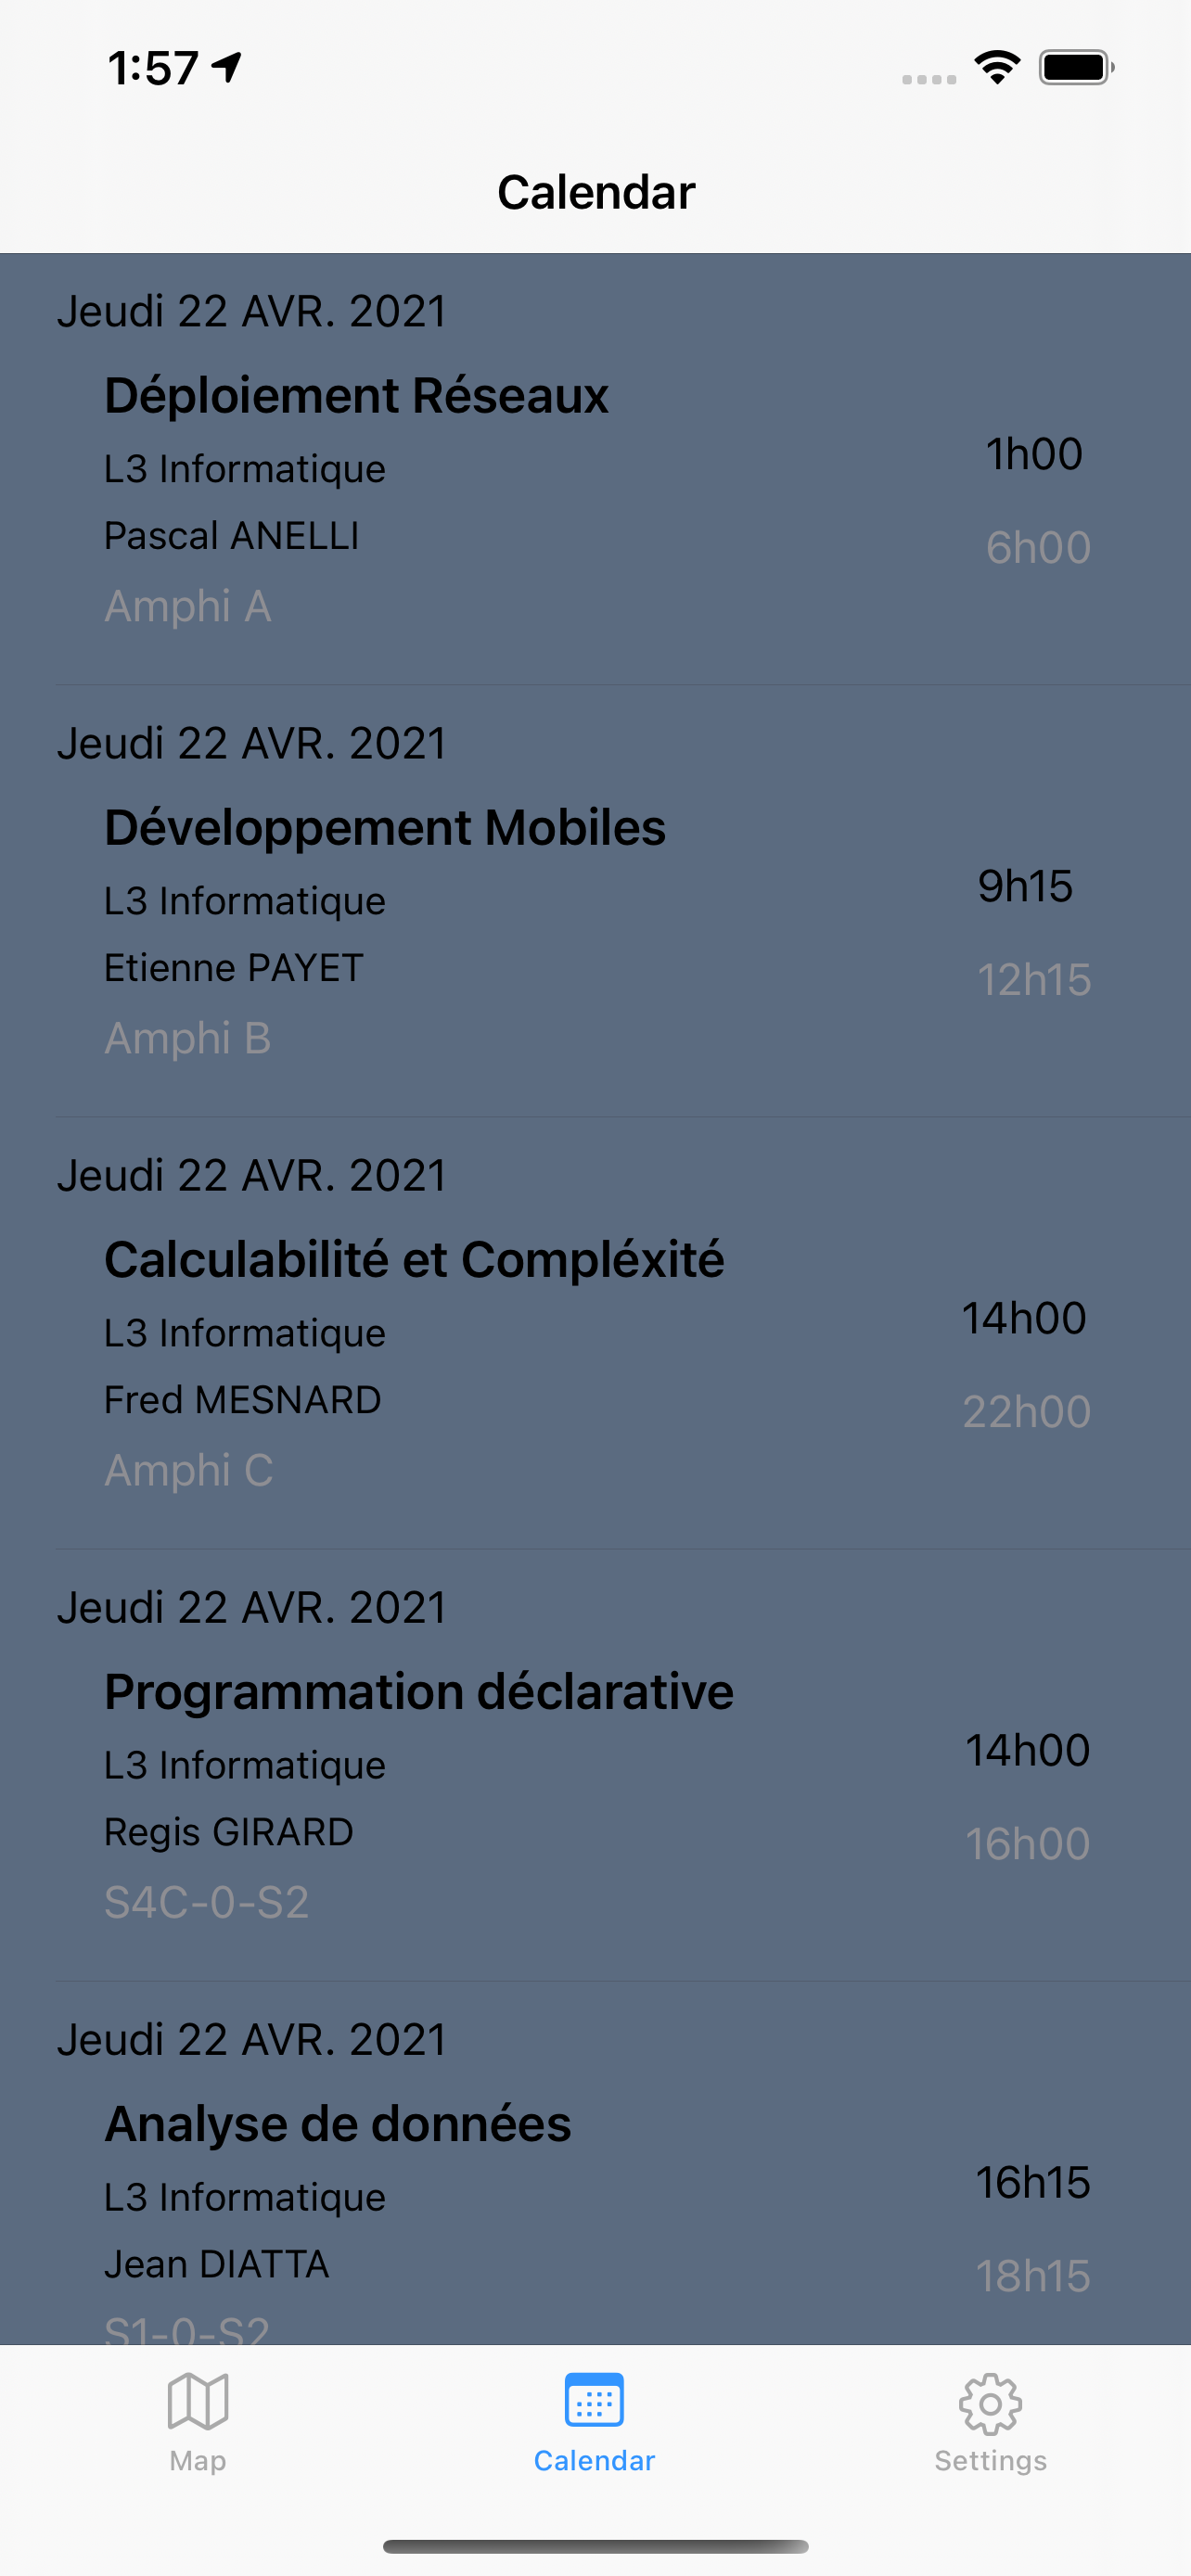
\includegraphics[width=50mm, scale=0.5]{calendar.png}
    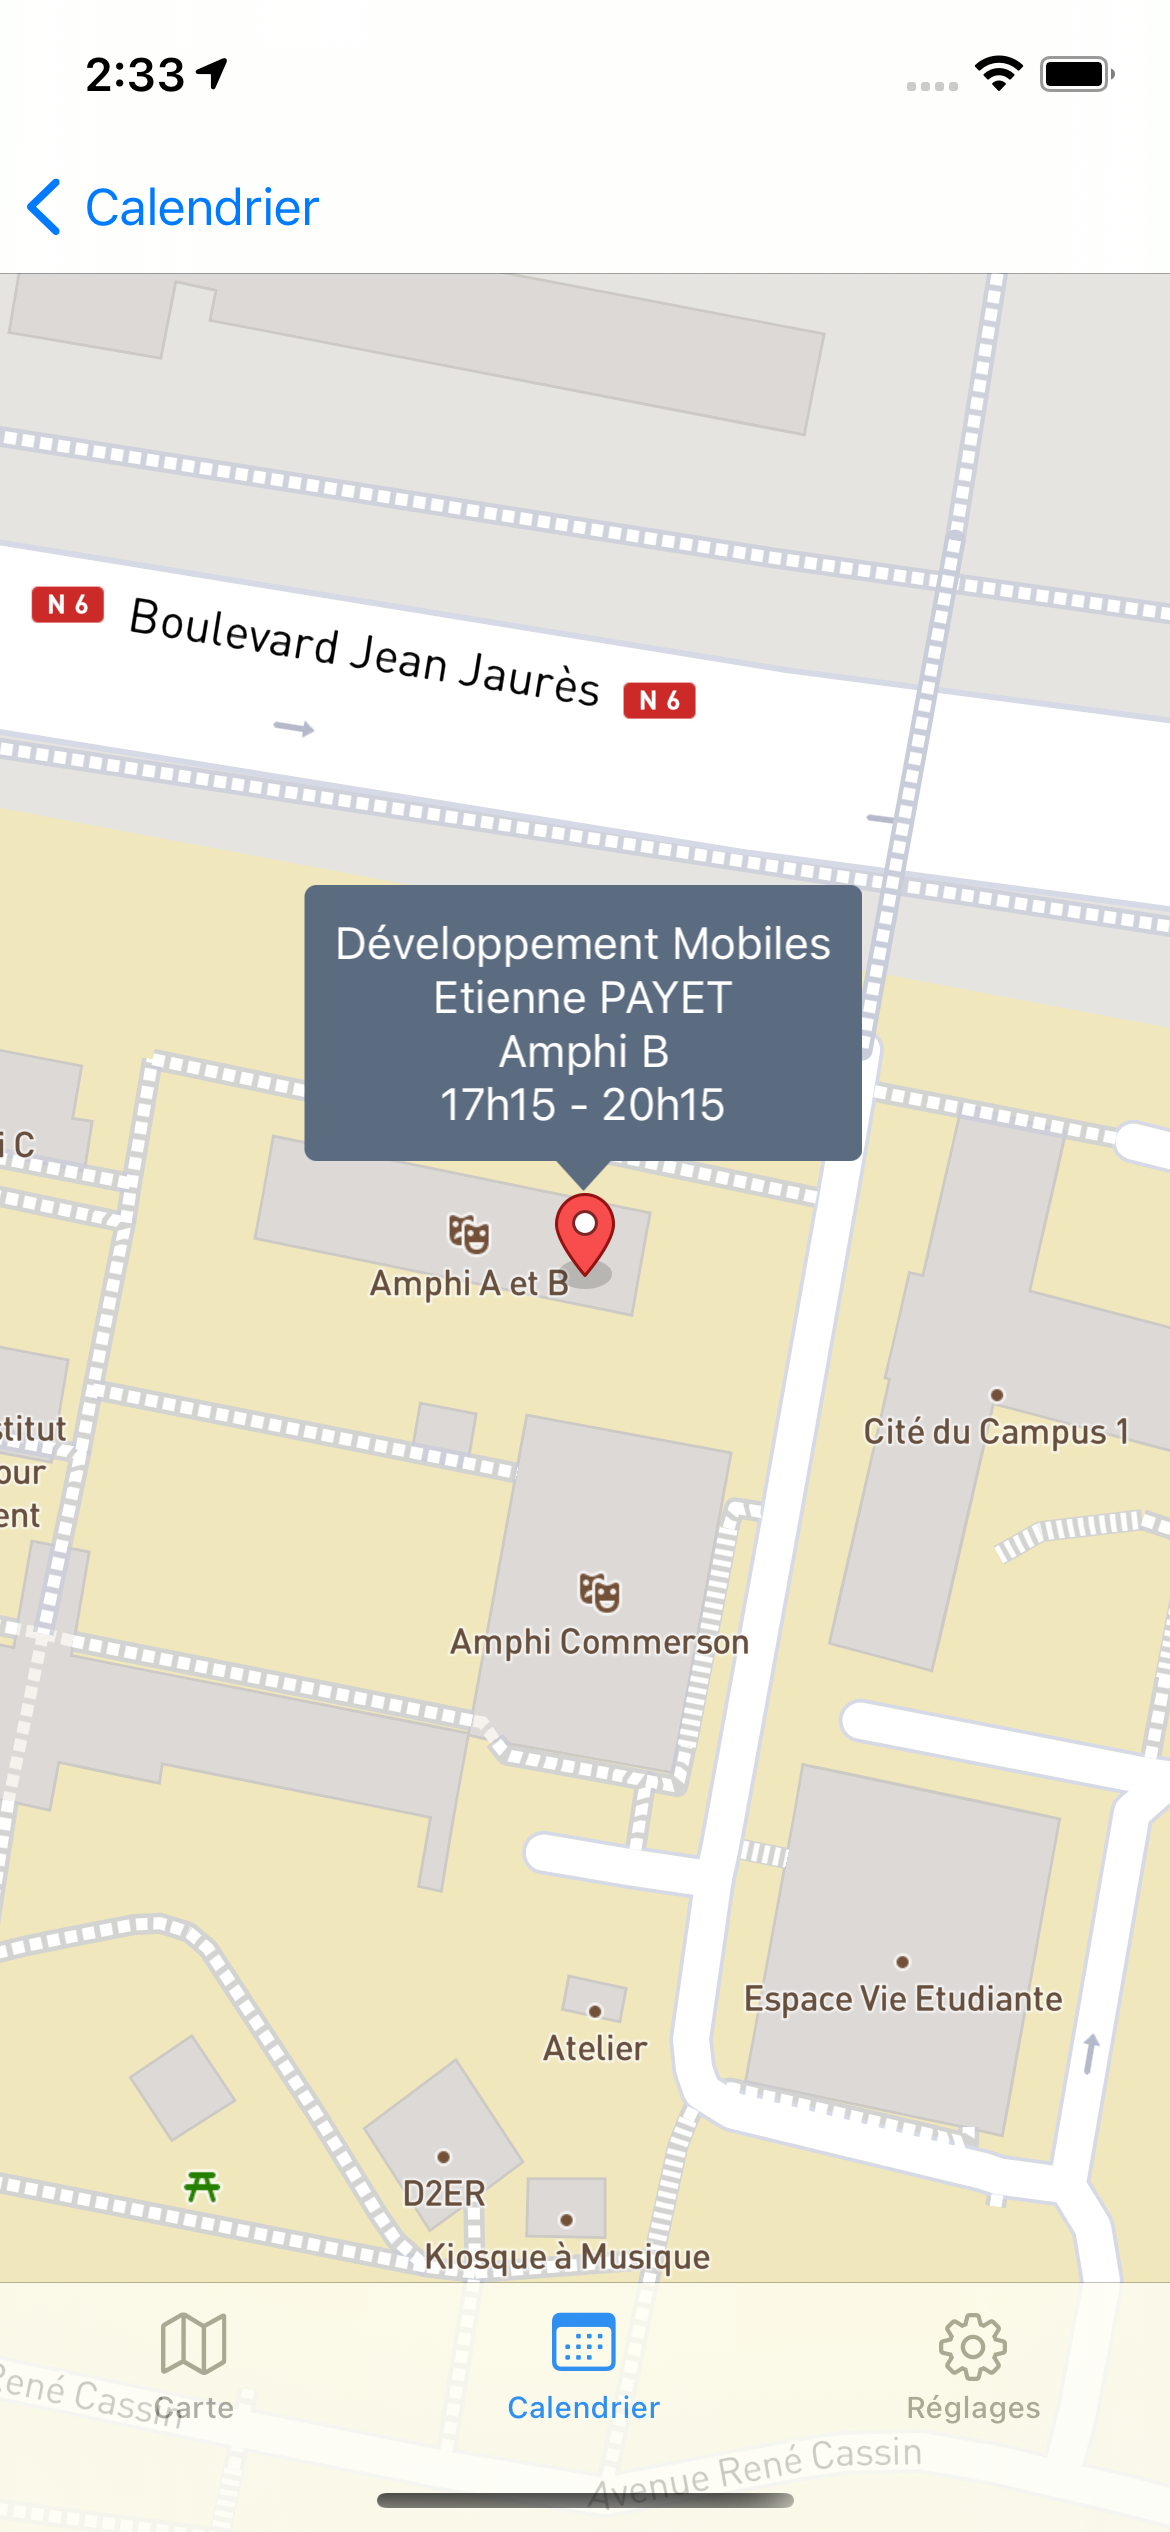
\includegraphics[width=50mm, scale=0.5]{calendar_position.png}
\end{center}



\newpage %% Passer a une autre page



\subsection{Présentation des paramétrages}
Enfin l'onglet des paramétres de l'application, présenté sous forme de liste(générer dynamiquement), permet à l'utilisateur de mieux s'approprier l'application et d'en apprendre plus sur elle. À travers cette l'onglet, nous voulions encore une fois mettre en valeurs notre volonté d'aidée les utilisateurs, tout en leurs apportant le maximum de confort. Pour cela, nous avons choisi de mettre en avant, pour cette première version de UnivMap, les paramètres suivants:

\begin{itemize}
    \item Le choix de la langue : La possibilité de choisir la langues de l'application est une option, qui nous semble toujours indispensable. Cette option augmente le confort certe, mais surtout permet aux public de différentes nationalité de l'utiliser.
    Pour cet option, l'utilisateur a le choix entre utiliser la même langue que son appareil, ou utiliser une des langues lister en-dessous.   

    \item Le choix du thème de l'application : le choix du thème de l'application permet à l'utilisateur de choisir la couleur de fonds, .
    
    \item Ainsi que l'assistance : En cas de problème, l'utilisateur est invité à contacter l'assistance par mail. Ainsi en cliquant sur assistance, puis envoyer il est rediriger dans une application de mail pour envoyer un mail à l'adresse qui y préfigure. 
    
    \item Mais aussi le mentions légales et la Confidentialité : Ces deux options sont présent à titre informatif, et sont indispensable à tout application qui ce veut accessible aux public. Dans ces deux partie doivent paraître respectivement la charte de protection des données personnelles, etc... et les CGU(conditions générales d'utilisation), etc...
    
    \item Et enfin, UnivMap : Cette option des paramétres est présente pour permet à l'utilisateur d'en apprendre plus sur UnivMap. Notamment, le but d'UnvMap, qui sont ses créateur, et suivre l'évolution de l'application. 
    
\end{itemize}

\vspace{10pt}   %espace

\begin{center}
    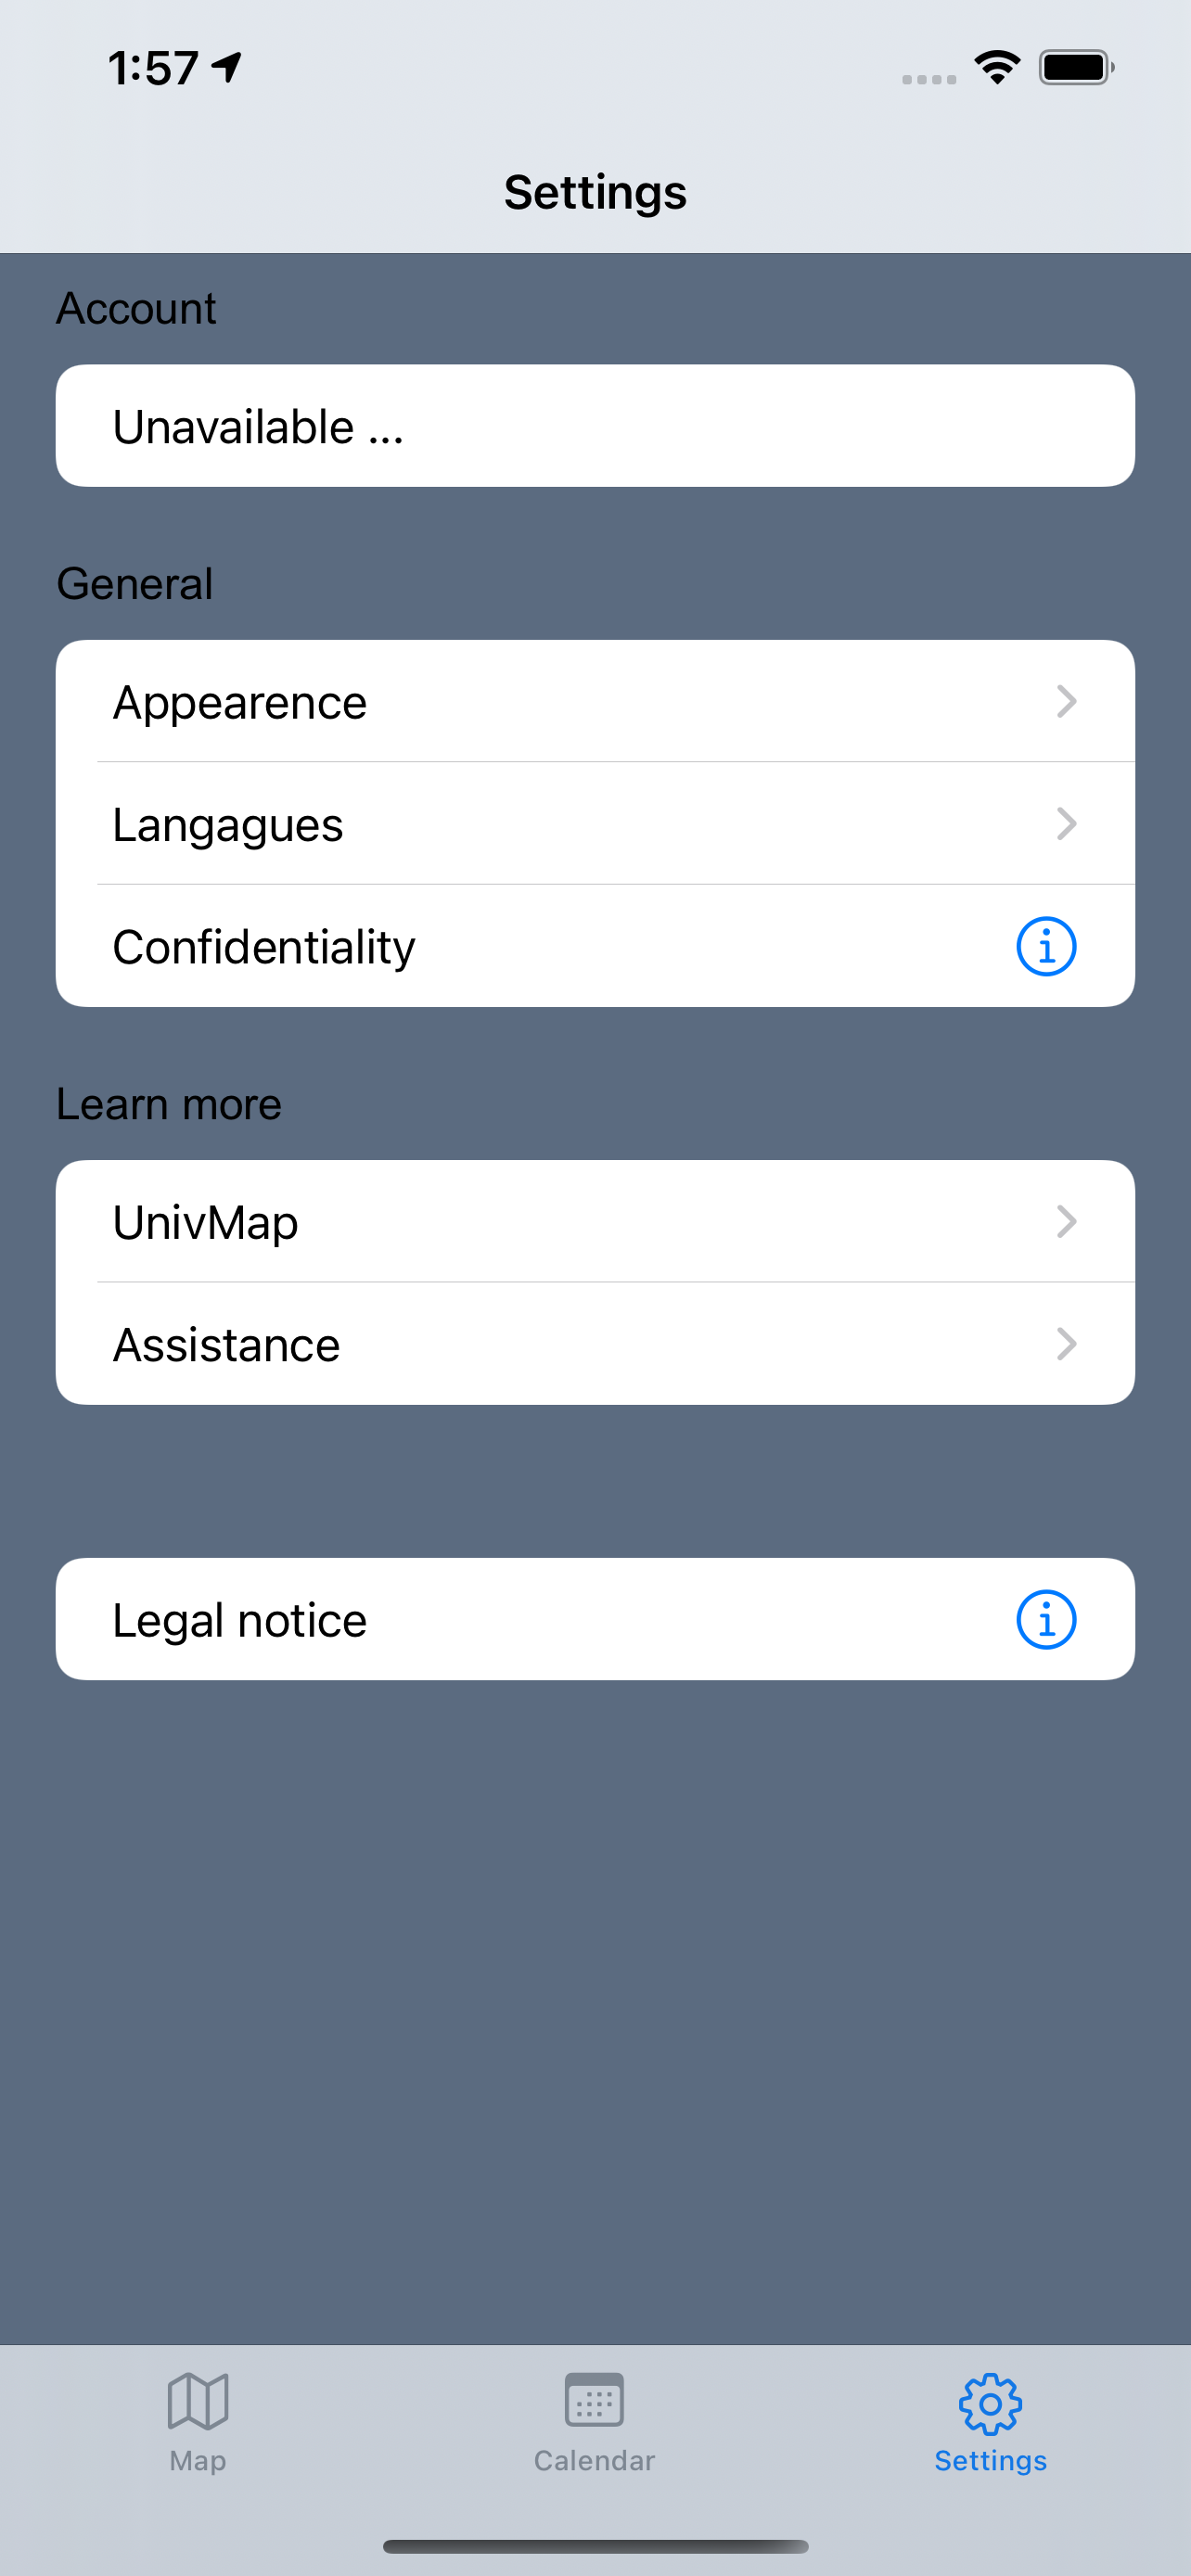
\includegraphics[width=35mm, scale=0.5]{setting.png}
    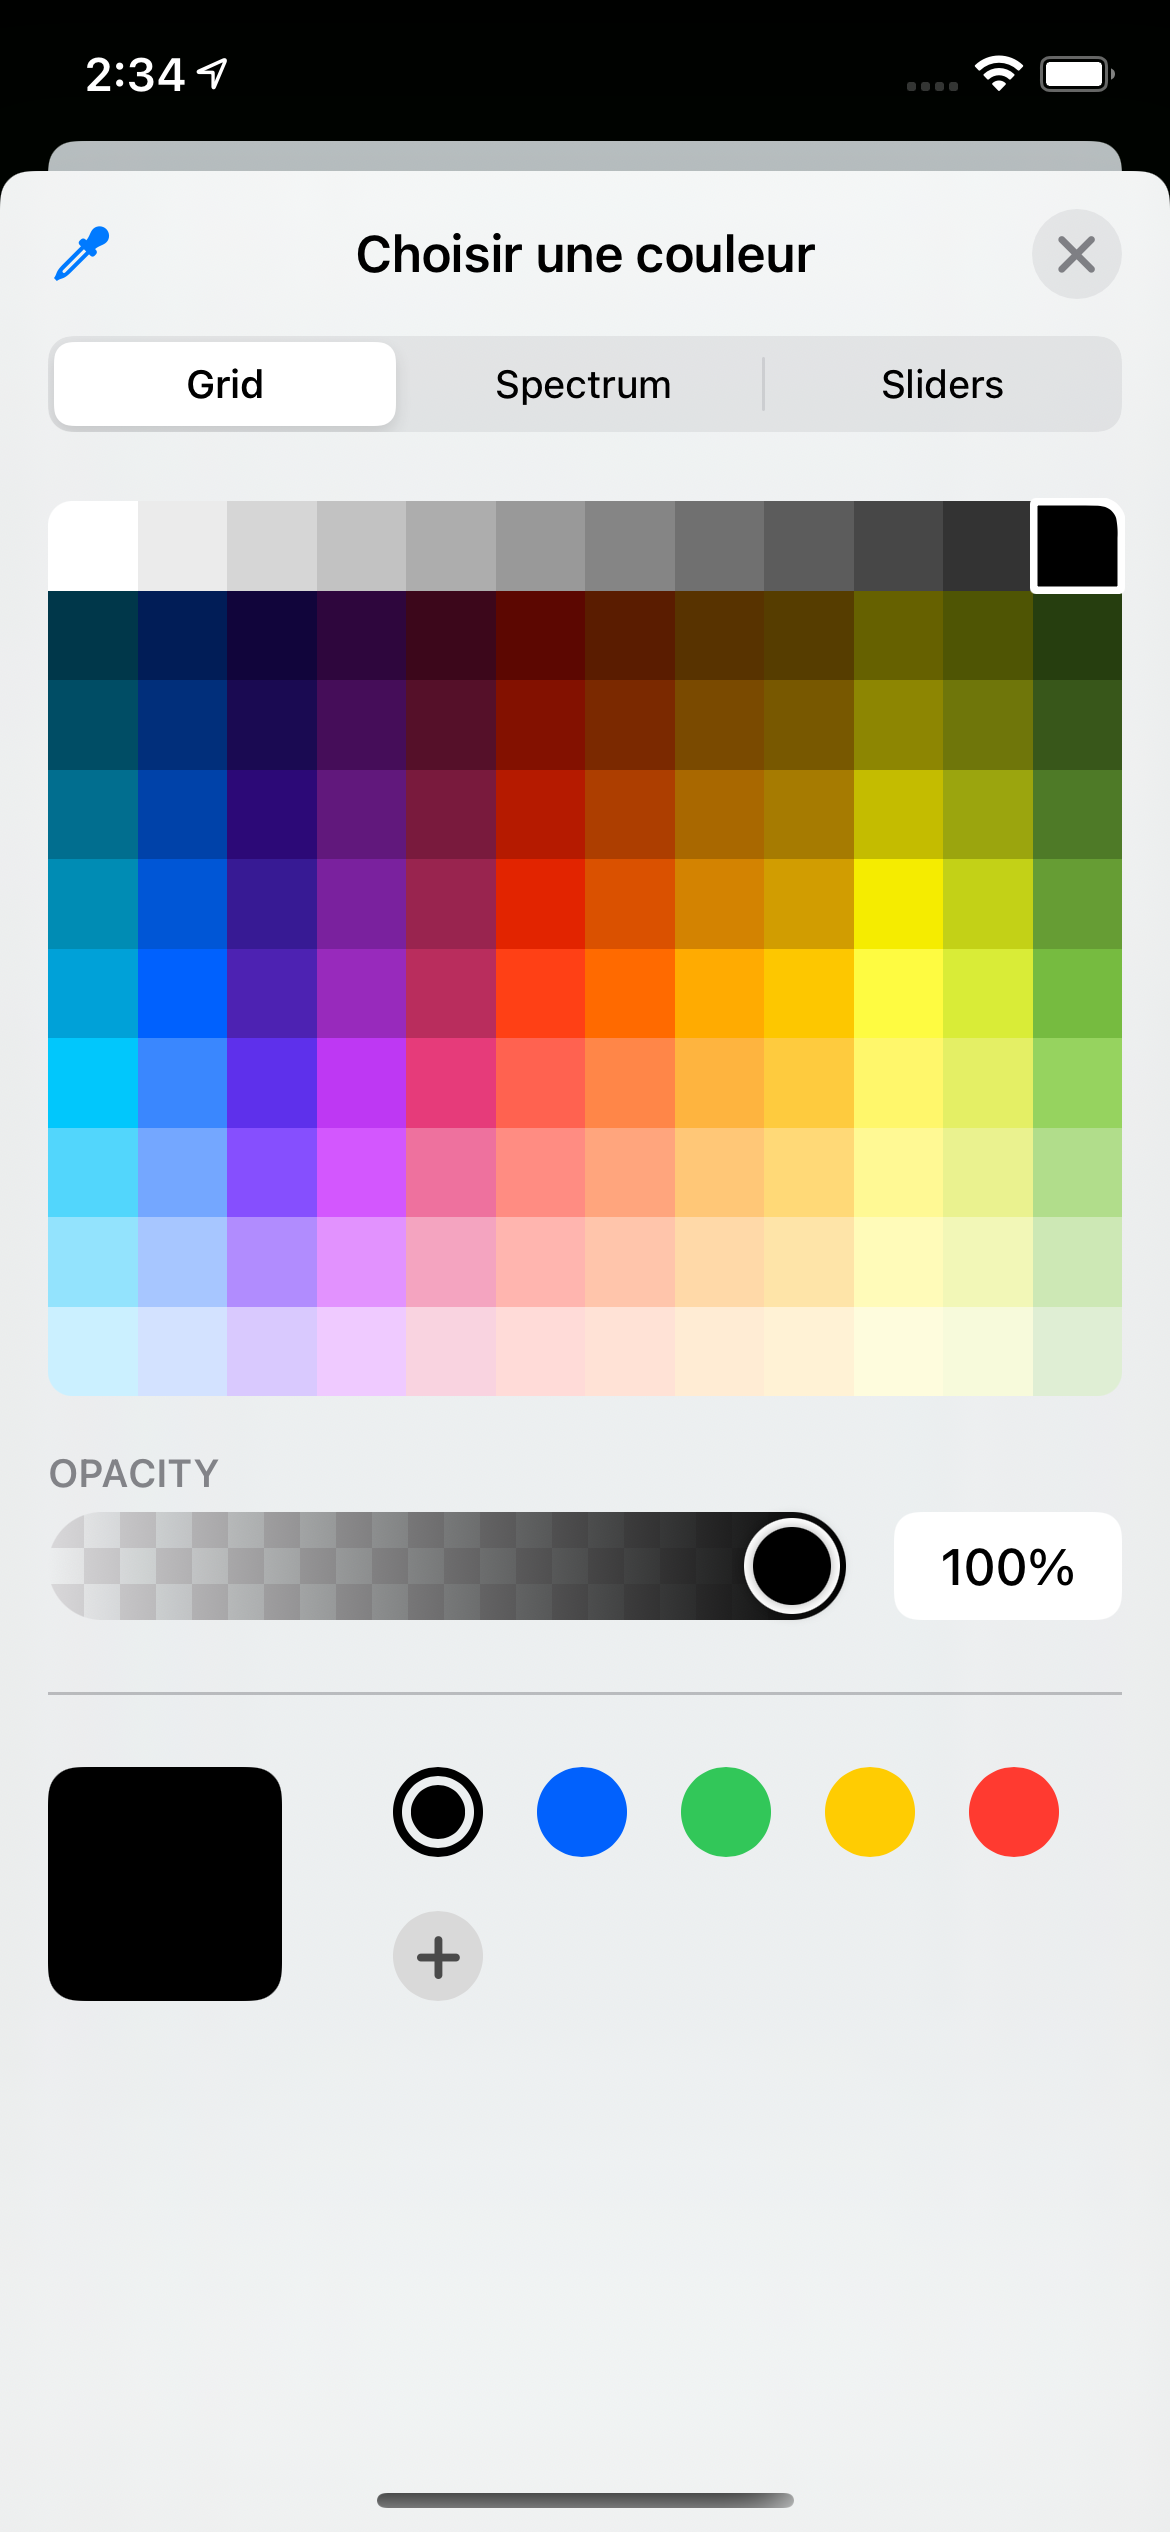
\includegraphics[width=35mm, scale=0.5]{setting_appearance.png}
    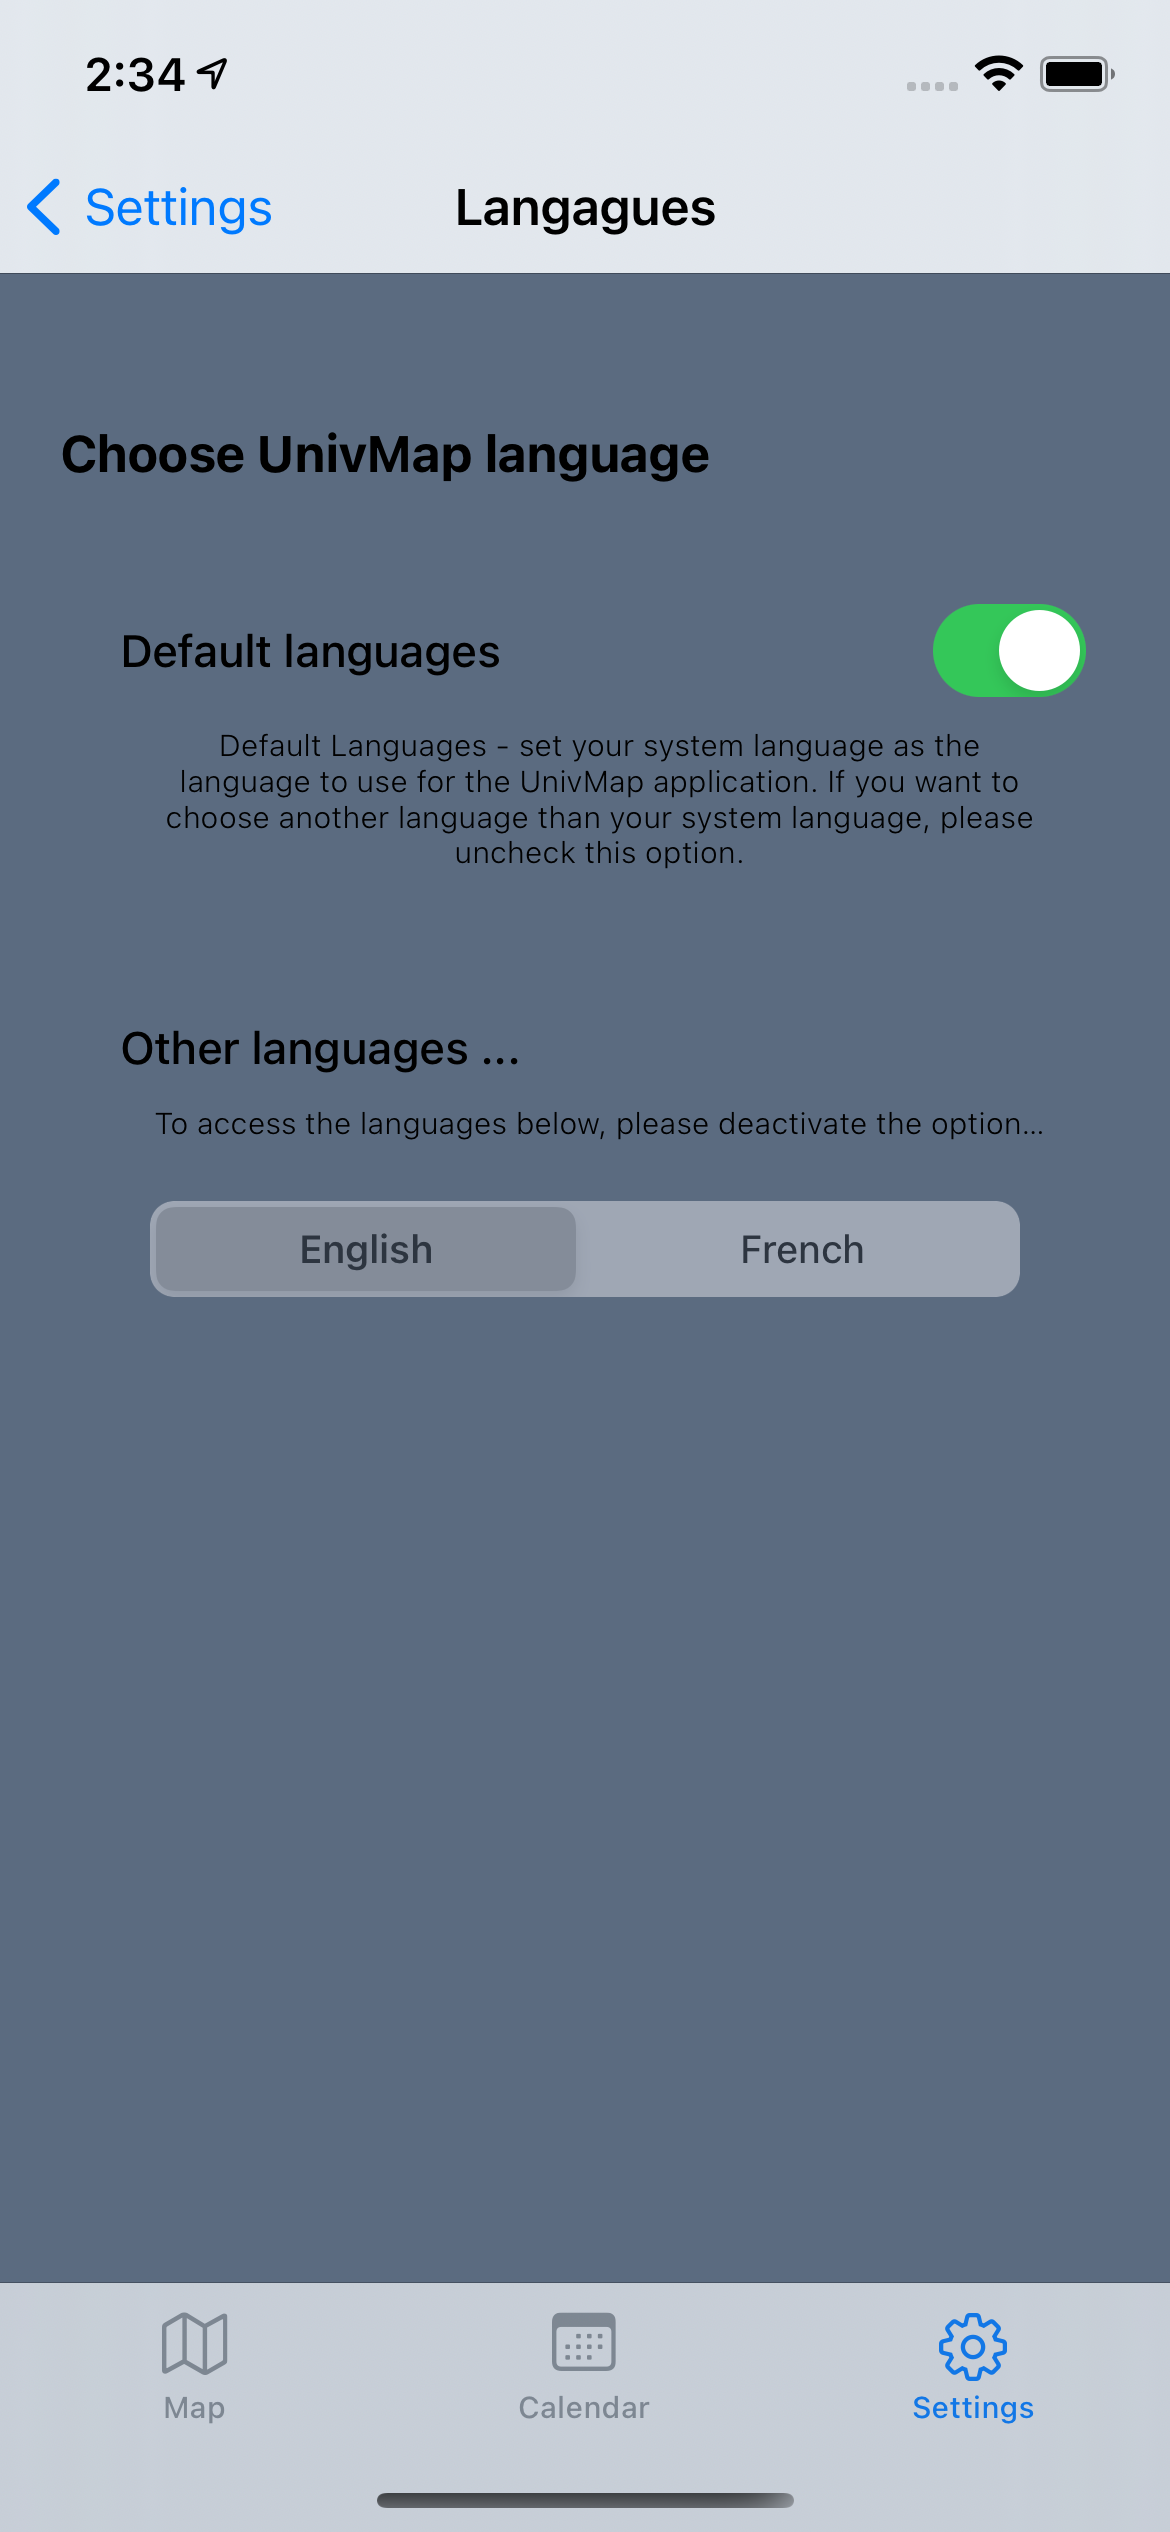
\includegraphics[width=35mm, scale=0.5]{setting_languageOn.png}
    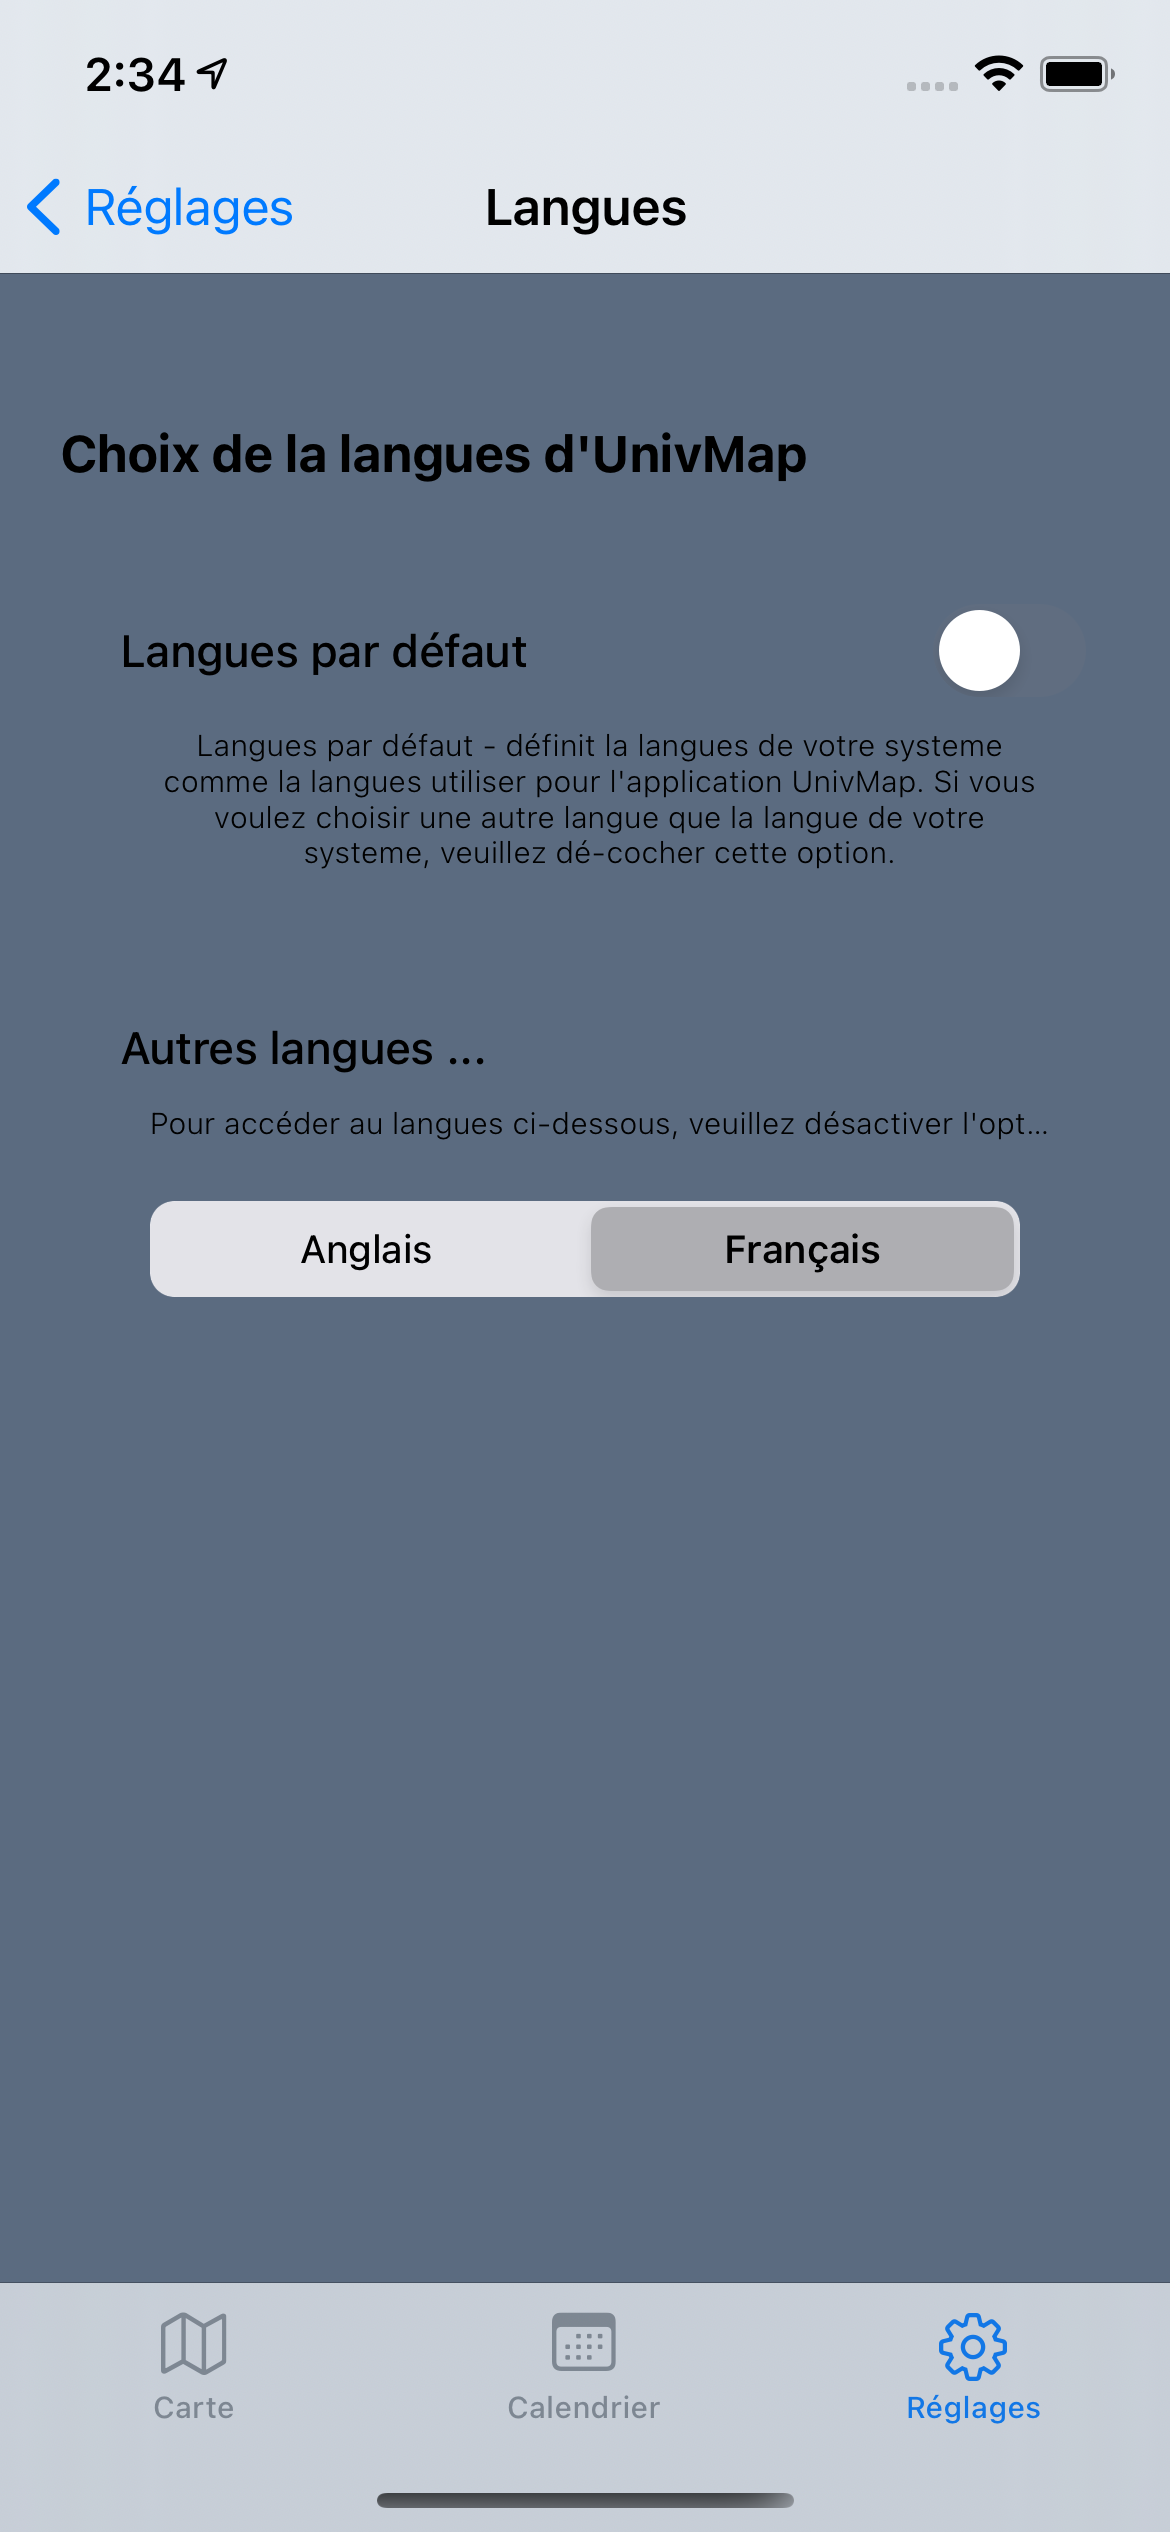
\includegraphics[width=35mm, scale=0.5]{setting_languageOff.png}
\end{center}



\newpage %% Passer a une autre page



\section{Architecture du code}
% \ref{...} permet de faire référence à un élément défini
% ailleurs dans le document (voir \label{...} plus haut).
UnivMap est une application iOS et Android développer respectivement en Swift et Java.


\subsection{Android} %% une sous-section
\label{subsection:Android} 


\subsubsection{Java : Ouverture à la base de donnée}
\label{subsubsection:Java : Ouverture à la base de donnée} 
Cette fonction permet d'ouvrir la connexion à Firebase et de récupérer les données selon la clé. Elle retourne
une liste d'objet en Callback.

\begin{verbatim}
    public void getAllData(ListPlanningCallback listPlanningCallback) {
        db.collection("planning")
                .get()
                .addOnCompleteListener(new OnCompleteListener<QuerySnapshot>() {
                    @Override
                    public void onComplete(@NonNull Task<QuerySnapshot> task) {
                        if (task.isSuccessful()) {
                            List<Planning> listLocal = new ArrayList<Planning>();

                            for (QueryDocumentSnapshot document : task.getResult()) {

                                String nom = document.getString("nom");
                                String filiere = document.getString("filiere");
                                String enseignant = document.getString("enseignant");
                                String hDebut = document.getString("hDebut");
                                String hFin = document.getString("hFin");
                                String mDebut = document.getString("mDebut");
                                String mFin = document.getString("mFin");
                                String salle = document.getString("salle");
                                String latitude = document.getString("latitude");
                                String longitude = document.getString("longitude");

                                Planning planning = new Planning(nom, filiere, enseignant...);
                                listLocal.add(planning);

                            }
                            listPlanningCallback.onCallback(listLocal);
                        } else {
                            Log.d(TAG, "Error getting documents: ", task.getException());
                        }
                    }
                });

    }

    public interface ListPlanningCallback {
        void onCallback(List<Planning> listPlanning);
    }
\end{verbatim}

\subsubsection{Java : Choix de la langue}
La première fonction permet de modifier la langue d'une chaine de caractère et la deuxième de récupérer la langue de l'appareil :

\begin{verbatim}
   
    public static void setLocale(Activity activity, String languageCode) {
        Locale locale = new Locale(languageCode);
        Locale.setDefault(locale);
        Resources resources = activity.getResources();
        Configuration config = resources.getConfiguration();
        
        if (Build.VERSION.SDK_INT >= Build.VERSION_CODES.JELLY_BEAN_MR1) {
            config.setLocale(locale);
        } else {
            config.locale = locale;
        }
        resources.updateConfiguration(config, resources.getDisplayMetrics());

    }

    public static String currentLanguage(){
        return Resources.getSystem().getConfiguration().locale.getLanguage();
    }

}\end{verbatim}



\subsection{iOS} %% une autre sous-section
\label{subsection:iOS} 


\subsubsection{Swift : Ouverture à la base de donnée}
\label{subsubsection:Swift : Ouverture à la base de donnée} 
Voici la même code en Swift que dans la section~\ref{subsubsection:Java : Ouverture à la base de donnée}.
Ici, il faut juste ajouter à listPlanning (initialiser en variable global).

\begin{verbatim}
db.collection("planning").getDocuments() { [self] (querySnapshot, err) in
            if let err = err {
                print("Error getting documents: \(err)")
            } else {
                
                for document in querySnapshot!.documents {
                    if let nom = document.data()["nom"] as? String,         //recup data selon clé
                        let filiere = document.data()["filiere"] as? String,
                        let enseignant = document.data()["enseignant"] as? String,
                        let hDebut = document.data()["hDebut"] as? String,
                        let hFin = document.data()["hFin"] as? String,
                        let mDebut = document.data()["mDebut"] as? String,
                        let mFin = document.data()["mFin"] as? String,
                        let salle = document.data()["salle"] as? String,
                        let latitude = document.data()["latitude"] as? String,
                        let longitude = document.data()["longitude"] as? String{
                    
                        self.listPlanning.append(Planning(nom: nom, filiere: filiere, ...))
                        
                        (...)
                    
                }
                
            }
        }


\end{verbatim}

\subsubsection{Swift : Choix de la langue}
Cette fonction permet de modifier la langue d'une chaine de caractère de trois manière différente :

\begin{itemize}
    \item Selon la langues passer en paramétre : Affiche toujours un texte dans une langue en particulier! 

    \item Selon la langue par défaut : Affiche toujours un texte dans la langues par défaut, c'est-à-dire la langue de l'appareil.

    \item Selon le choix de l'utilisateur : Affiche le texte dans la langue choisit par l'utilisateur.
\end{itemize}

\begin{verbatim}
    extension String {
    func localized(str:String?) -> String{
        if let language = str{
            let path = Bundle.main.path(forResource: language, ofType: "lproj")
            let bundle = Bundle(path: path!)
            return NSLocalizedString(self, tableName: "Localizable", bundle: bundle!, value: self,
            		 comment: "nil")
        }
        if(UserDefaults.standard.bool(forKey: "switchState")){
            return NSLocalizedString(self, tableName: "Localizable", bundle: .main, value: self,
            		 comment: "nil")
        }
        let path = Bundle.main.path(forResource: UserDefaults.standard.string(forKey: "language"), 
        				ofType: "lproj")
        let bundle = Bundle(path: path!)
        return NSLocalizedString(self, tableName: "Localizable", bundle: bundle!, value: self,
        				 comment: "nil")
    }
}  
\end{verbatim}


\newpage %% Passer a une autre page


\section{Quelques points délicats/intéressants}

Durant le développement de notre application, nous avons rencontrés des difficultés concernant la prise en main
de nouveau outils de travail tels que Git.
De plus, l'implémentation de l'API Mapbox et de \textit{Firebase}~\cite{firebaseDoc} à beaucoup ralenti
le développement sur iOS. En effet, \textit{Firebase}~\cite{firebaseDoc} étant développer par Google, son importation
était une épreuve sur Xcode. Afin d'installer les dépendances requises sur iOS, nous avons du passé par
le gestionnaire de dépendances \textit{CocoaPods}~\cite{cocoapodsDoc}.
Malgré tous ces difficultés et après avoir pris en main, l'API Mapbox nous a permis de finir ce projet dans les temps.
Mapbox étant très complet, possèdent ses propres classe permettant aux développeur de l'intégrer facilement dans leurs
projets.
Concernant \textit{Firebase}~\cite{firebaseDoc}, son utilisation est plus aisé en Swift. En effet, Swift permet
l'ajout de valeur dans une liste d'objet déclarer globalement. Contrairement à Java, ou il a fallu passé par une
fonction callback (voir section~\ref{subsubsection:Java : Ouverture à la base de donnée}) pour récupérer les données.
La traduction de l'application, en iOS révèle la puissance des extensions qui permet de rajouter des fonctions, structures, etc... Et cela même à des classes normalement inaccessibles (code sources) comme la classe String. Néanmoins, il était plus simple de gérer la traduction en java. La gestion de la traduction et de l'apparence de l'application, nous a confronté au cycle de vie (des view/activity) des différentes plateformes. Et l'utilisation des données persistances sous forme de couple clé, valeurs pour enregistrer des petit donnée (préférences utilisateurs), est remarquable.  Les données persistantes nous ont même permis de détecter la première utilisation de l'application, pour exécuter du code qu'une seule fois.

\subsection{UnivMap 2.0 à suivre}
À la fin du développement de notre application,  bien qu'elle soit fonctionnelle certains améliorations sont à venir, tel que :
\begin{itemize}
    \item l'ajout du choix de la fillière;

    \item l'ajout de notification lorsque le calendrier est modifier;

    \item l'ajout d'un onglet accueil avec des redirections vers les autres platforms de l'Université et l'affichage d'évèments;
    
    \item l'ajout de filtre sur la carte.
    
\end{itemize}



\section{Conclusion}


%%% La bibliographie:
\bibliographystyle{plain}
\bibliography{ma_biblio}

\end{document}



